\subsection{Attacks}
This subsection will deal with existing attacks that can be used to gain control over a process.
\begin{figure}[h]
\centering
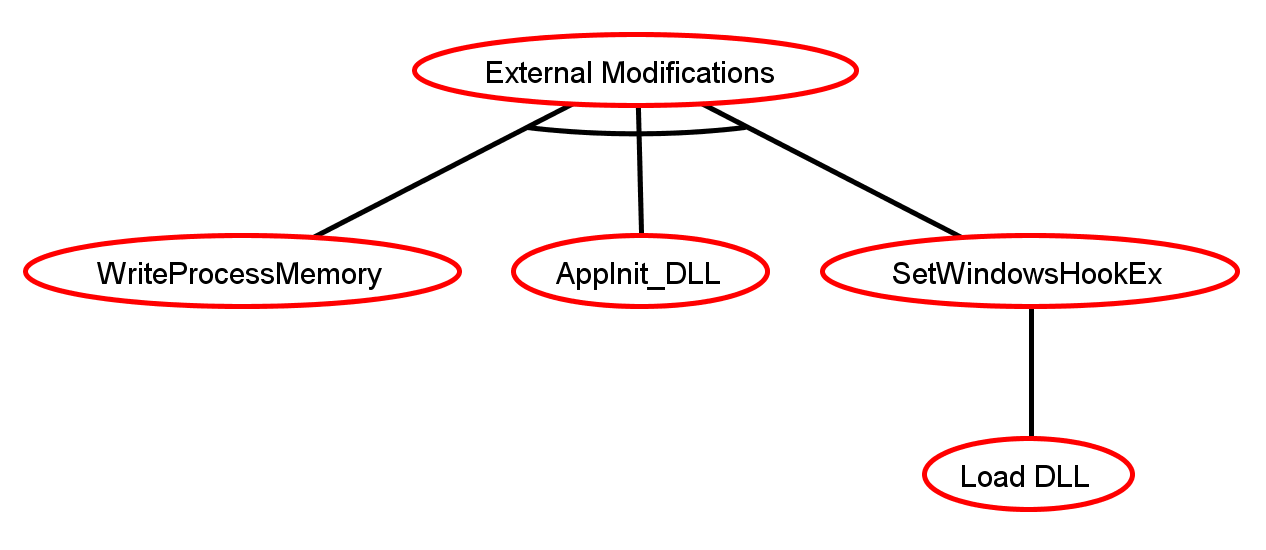
\includegraphics[scale=0.35]{sections/adtrees/ExternalModificationsWithoutDefenses.png}
\caption{This attack tree shows all possible external modifications to the original software.}
\label{fig:attacks_external}
\end{figure}
\subsubsection{\emph{Registry} based injection}
\emph{Registry} based injection uses a special \emph{Registry} key\footnote{The \emph{Registry} key can be found at \syscall{HKEY\_LOCAL\_MACHINE\textbackslash Software\textbackslash Microsoft\textbackslash\allowbreak Windows NT\textbackslash CurrentVersion\textbackslash Windows}} that can be used to inject \gls{DLL} files into almost any process. For that reason the shown attack tree in Figure~\ref{fig:attacks_external} lists this technique under the group of \gls{DLL} injections in node [1.2.1]. \glspl{DLL} can be added by writing the full path to the file into this \emph{Registry} key, with multiple paths separated by semicolons. To make this injection technique work, two conditions have to apply:
\begin{enumerate}
\item The \gls{DLL} file is having a security descriptor that allows execution. Otherwise the \gls{DLL} will not get loaded into the target process.
\item The \gls{MSDN} \cite{msdn_appinitdlls} lists the usage of \syscall{User32\allowbreak.dll} in the target process as a requirement or otherwise the \glspl{DLL} listed in the \emph{Registry} will not get loaded.
\end{enumerate}
However, these two conditions are easy to fulfill. The first condition is by default true, because the default security descriptor on \gls{DLL} files allow execution. Active interaction by other programs or the user is required to change the security descriptor. The second condition is most of the time fulfilled. \syscall{User32.dll} is used in almost every process and in general it can be assumed that the \gls{MSDN} requirement is fulfilled. To make this attack work, a second \emph{Registry} key, \syscall{LoadAppInit\_DLLs}, has to be changed to value 1, in order to activate this \emph{Registry} based injection. By default this value is set to 0 and cannot be changed without admin privileges.
Defending against this kind of attack is comparably easy, by checking \syscall{AppInit\_DLLs} value and enumerating all loaded modules (\glspl{DLL}). If a match is found and considered to be unwanted, it can be unloaded or as a safety measurement the application is terminated. As for \emph{Google Chrome}, there is no validation currently in place and \emph{Registry} based injection can be used to load arbitrary \gls{DLL} files.
\subsubsection{\syscall{SetWindowsHookEx} Injection}
Another way besides \emph{Registry} based injections is using the \syscall{SetWindowsHookEx} function of the \emph{Windows} \gls{API} to inject a \gls{DLL} file. It requires no special privileges to be executed and can be used to  hook into a specific application or being system wide. A hook in this context is a callback function that gets executed whenever a certain event is occurring. In terms of \syscall{SetWindowsHookEx}, there are according to the \gls{MSDN} \cite{msdn_setwindowshookex} 15 different possible types of events that can be registered for, of which some can only be system wide. The hook procedure that is required as parameter for \syscall{SetWindowsHookEx} has to be located in a \gls{DLL} file. The \gls{DLL} to be injected is loaded by the operating system into the current process, to make the specified callback function available. An example code is shown in Appendix~\ref{appendix:setwindowshookex}. As this attack is also a based on \gls{DLL} injections the attack tree of Figure~\ref{fig:attacks_external} lists this attack under [1.2.2] in external modifications. 

\medskip

The \gls{DLL} will not get loaded into the target process until the event is triggered and the registered hook is called for the first time. The callback procedure gives different opportunities to make use of this created situation. An additional thread can be started from the callback procedure or the called driver entry function to make the injection independent of the hook callback function. As this module and especially any created thread are running in the context of the remote process, the \gls{DLL} code has full access to the process' memory. Internal memory modifications can be performed, which will get explained in Section \ref{sec:internal_modifications}. As well as for \emph{Registry} based injections, \emph{Google Chrome} does not prevent \syscall{SetWindowsHookEx} \gls{DLL} injections.
\subsubsection{DLL Replacement}
The last missing DLL injection technique of the given attack tree in Figure \ref{fig:attacks_external} is DLL Replacement. The idea is to replace an existing DLL file with a patched or completely different DLL, which is possible due to the windows internal concepts. Every DLL exports functions that can be called from a program. The attack know creates a new DLL file, that exports the same functions and internally redirects all calls to the original DLL file. Therefore the functionality of the application stays the same and the attack is harder to detect. It is now possible to use on of the exported functions to execute other, new code that performs malicious activities.

\subsubsection{\syscall{WriteProcessMemory} external modifications}
\syscall{WriteProcessMemory} is just like the previously discussed \syscall{SetWindowsHookEx} a function available through the Windows API. This function allows to write into the virtual memory of a target process and allows modifying existing data or code. There are several ways to make use of this function, one of them being DLL injection with the \syscall{CreateRemoteThread} and \syscall{LoadLibrary} functions. 

\paragraph{\syscall{CreateRemoteThread} DLL Injection}
DLLs can be loaded into a target process by loading its path into the target memory with \syscall{WriteProcessMemory} and creating a new thread via \syscall{CreateRemoteThread} that calls \syscall{LoadLibrary}. This kind of attack can be used on any process running under the same integrity level and therefore is very widely used in game cheating. At first, a handle to the target process is requested via \syscall{OpenProcess} with \syscall{PROCESS\_VM\_WRITE} and \syscall{PROCESS\_VM\_OPERATION} access rights, which are required to execute the important \syscall{WriteProcessMemory} function. If the permissions are missing, \syscall{WriteProcessMemory} is not able to modify the virtual memory of the target process. Virtual memory protection flags don't have to be changed manually, as this is already happening inside \syscall{WriteProcessMemory}. After that, a large enough amount of memory is allocated inside the target process with \syscall{VirtualAllocEx}, to hold the full path of the DLL. Next \syscall{WriteProcessMemory} is used to transfer the DLL path into the target memory space and finally the injection can be completed by calling \syscall{CreateRemoteThread}, which finally loads the DLL with the \syscall{LoadLibrary} function. The allocated memory segment is used as a parameter for the \syscall{LoadLibrary} function call. With the now loaded DLL, arbitrary code can get executed by the DLL, either via using \syscall{CreateRemoteThread} again or via the DLLs entry point.
An example of a very basic DLL injection using \syscall{WriteProcessMemory} and \syscall{CreateRemoteThread} can be found in appendix \ref{appendix:writeprocessmemory}. Again, chrome shows no existing defense mechanisms against direct memory modification.

A second way to make use of \syscall{WriteProcessMemory} is modifying the targets code inside memory, to execute different instructions than intended. This technique is also commonly known as function hooking or function detouring, which is described in the next paragraph. 
\paragraph{Function detouring}
\begin{figure}[!htbp]
	\centering
	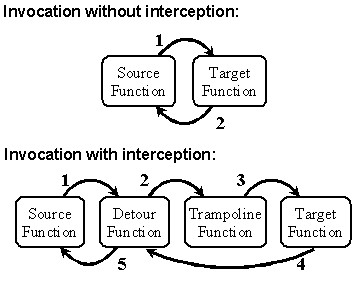
\includegraphics[scale=0.7]{sections/background/attacks/fig_detours.png}
	\caption{This figure shows the change in control flow of a detoured function \cite{detours}}
	\label{fig:detours}
\end{figure}


Function detouring has been greatly simplified by the Detours\cite{msdetours} library of Microsoft, but can also be achieved by memory modification with \syscall{WriteProcessMemory} or assembly code. Figure \ref{fig:detours} shows the difference between a function before and after detouring. The function call at the top shows a invocation without interception. The source function calls the target function without any indirection and after the code of the target function has been executed, returns to the calling source function. Detouring makes use of this structure by placing a detour and a trampoline function in between these calls. The source function will now use an indirect call to the target function, by first calling the detour part, which gives space to execute arbitrary code. To do that, a \syscall{jmp} instruction is placed at the beginning, and the original instructions are saved and copied to the trampoline function. After that, the detour function continues with the trampoline function, which executes the copied instructions and ensures that the target function works as if there was no detour placed. Finally, the whole function stack will return, this time skipping the trampoline function, as it was just used to hold the copied instructions. 

A detection of this technique is very difficult and can only be obtained by measuring the performance of called functions. If execution then takes in average exceptionally longer, there might be a detoured function. It is however impossible to make this detection reliable for all functions, as the systems unexpectable scheduling and load influence the resulting performance.

\subsubsection{Buffer overflows}
Buffer overflows are among the most severe security problems of modern applications, as they are hard to detect, and are introduced by simple programming errors that weren't previously found in testing and quality assurance steps. Even though they are hard to find, once used they allow the attacker to hopefully execute arbitrary code. If code execution is not possible, sensitive information might get revealed. One of the most severe examples of the past was the so called "Heathbleed bug", which affected millions of servers worldwide, as it was present in the much used OpenSSL library. Even though the attacker couldn't execute code, he was able to get sensitive information about the SSL certificates private key and thus break any security put in place by the SSL protocol. This attack is the last one of Figure \ref{fig:attacks_external} and also a external modification. In contrast to the other previously shown attacks there are several countermeasures existing to mitigate the resulting exploit, which will be discussed in chapter \ref{sec:defenses}.

\subsubsection{Internal modifications}
\label{sec:internal_modifications}
\begin{figure}[h]
\centering
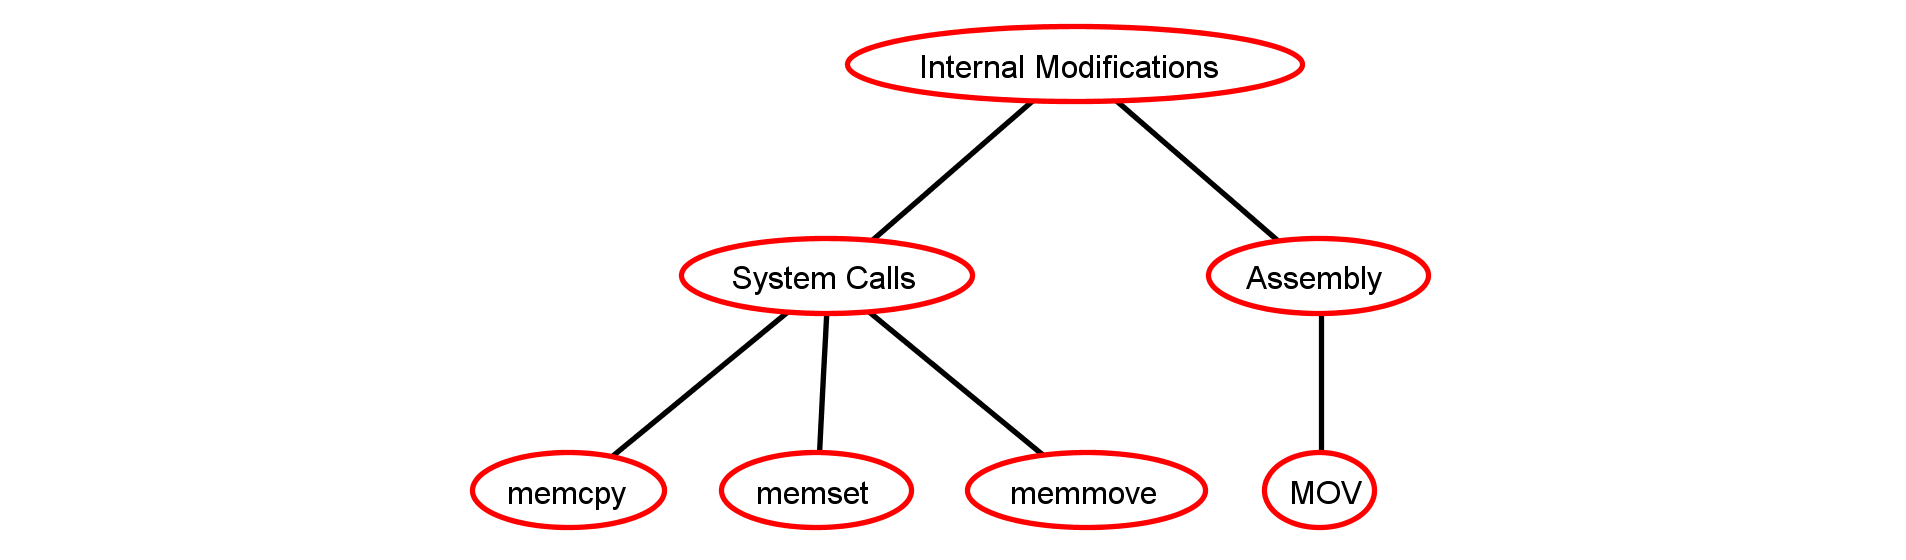
\includegraphics[scale=0.45]{sections/adtrees/InternalModificationsWithoutDefenses.png}
\caption{This attack tree shows possible attacks that are grouped under internal modification.}
\label{fig:attacks_internal}
\end{figure}
A group of attack is internal modifications which is in contrast to external modifications occurring from inside the process virtual memory. As the attacker is already inside the virtual memory, modification is easier and less restricted then the previously shown external modifications. The attacker can make use of existing functions like \syscall{memcpy} or \syscall{memset}, to modifiy the values inside memory, without having to use the indirection via \syscall{WriteProcessMemory}. Besides the present \syscall{mem*} functions, the attacker can also make use of assembly code. Figure \ref{fig:attacks_internal} shows this type of attack. The assembly part outlines the \syscall{mov} instruction, as it is mainly used to detour functions without the usage of exported API functions.

The shown attacks are combined in Figure \ref{fig_attacks}, containing now both parts of attacks, external and internal modifications.
\begin{figure}[!h]
	\centering
	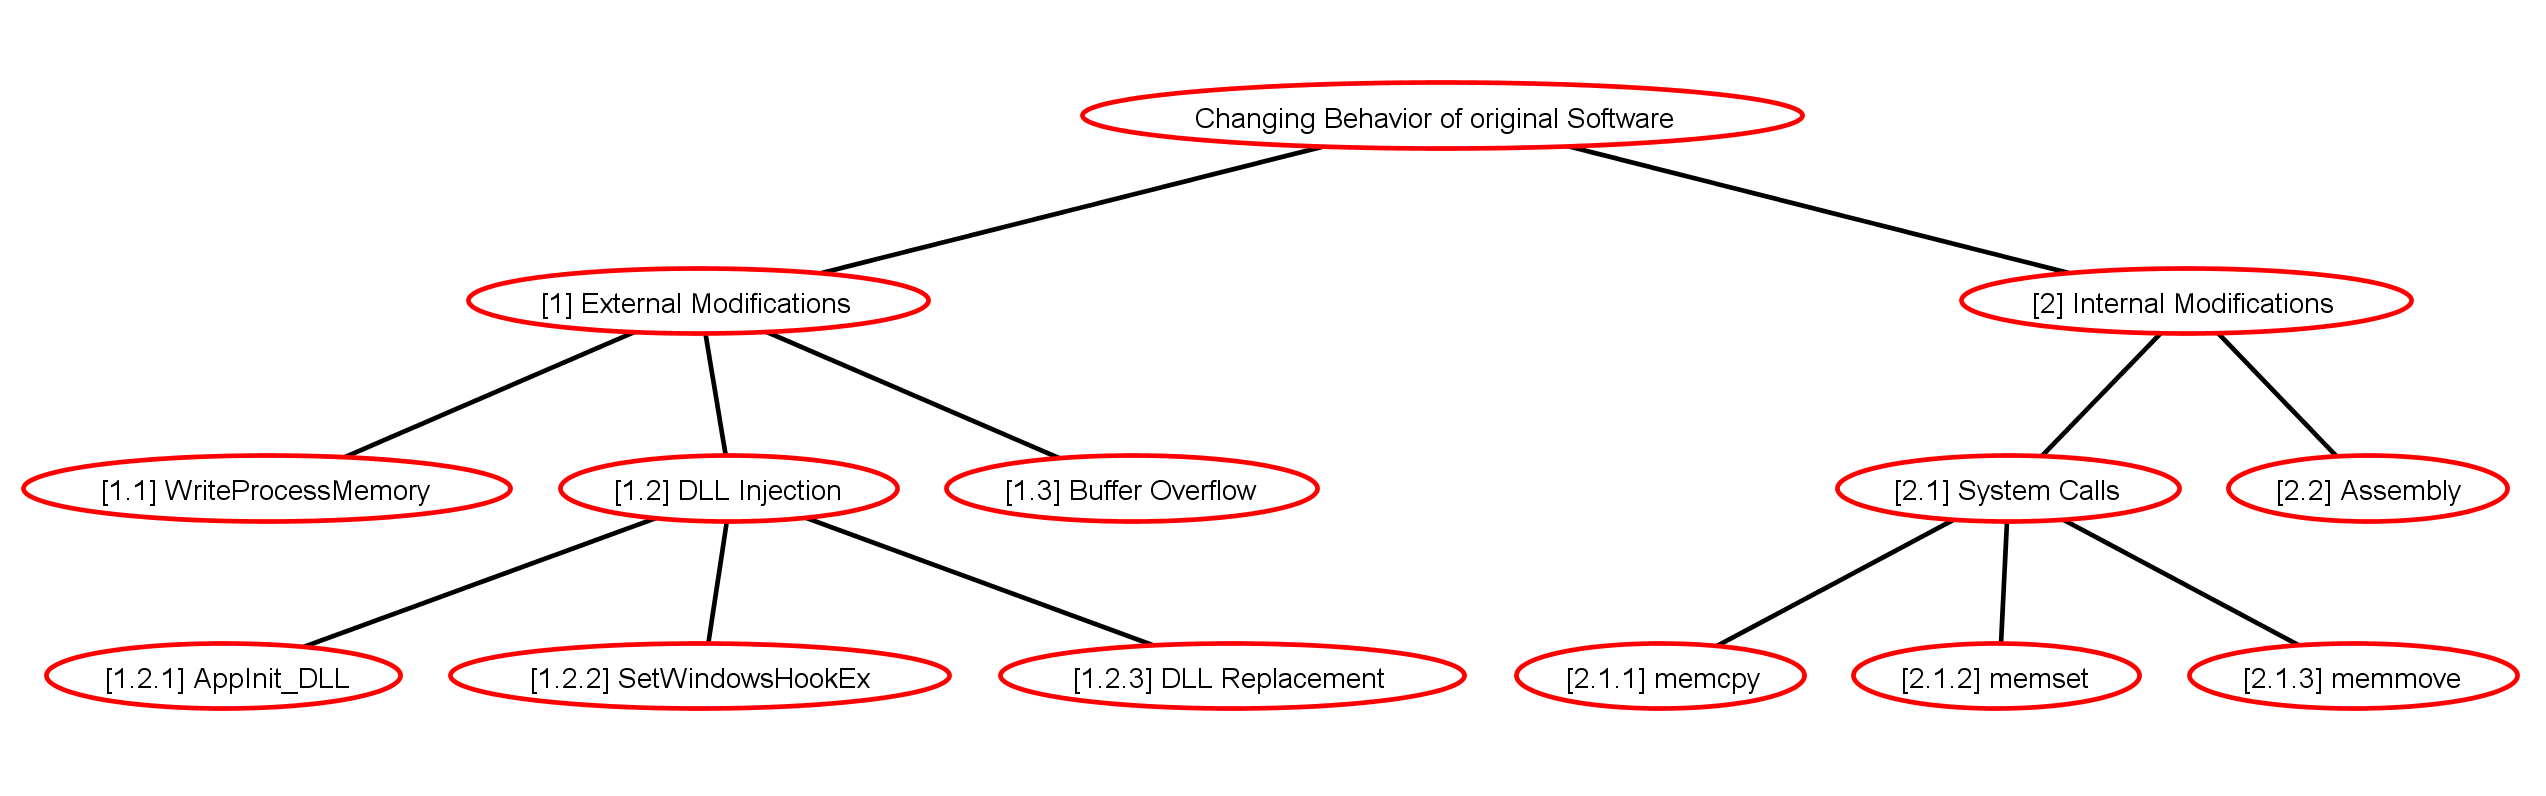
\includegraphics[angle=90,height=\textheight,keepaspectratio]{sections/adtrees/ProcessVirtualMemoryWithoutDefenses.png}
	\caption{An attack tree combining all of the shown attacks}
	\label{fig:attacks}
\end{figure}
